\documentclass{article}

\usepackage{graphicx}
\usepackage{tikz}
\usepackage{tikzsymbols}
\usetikzlibrary{calc,patterns,shapes.geometric}
\pagestyle{empty}
\usepackage[margin=0pt]{geometry}
\geometry{papersize={14in,12in}}

\def\centerarc[#1](#2)(#3:#4:#5){\draw[#1] ($(#2)+({#5*cos(#3)},{#5*sin(#3)})$) arc (#3:#4:#5);}

\begin{document}
	\begin{figure}
		\centering
		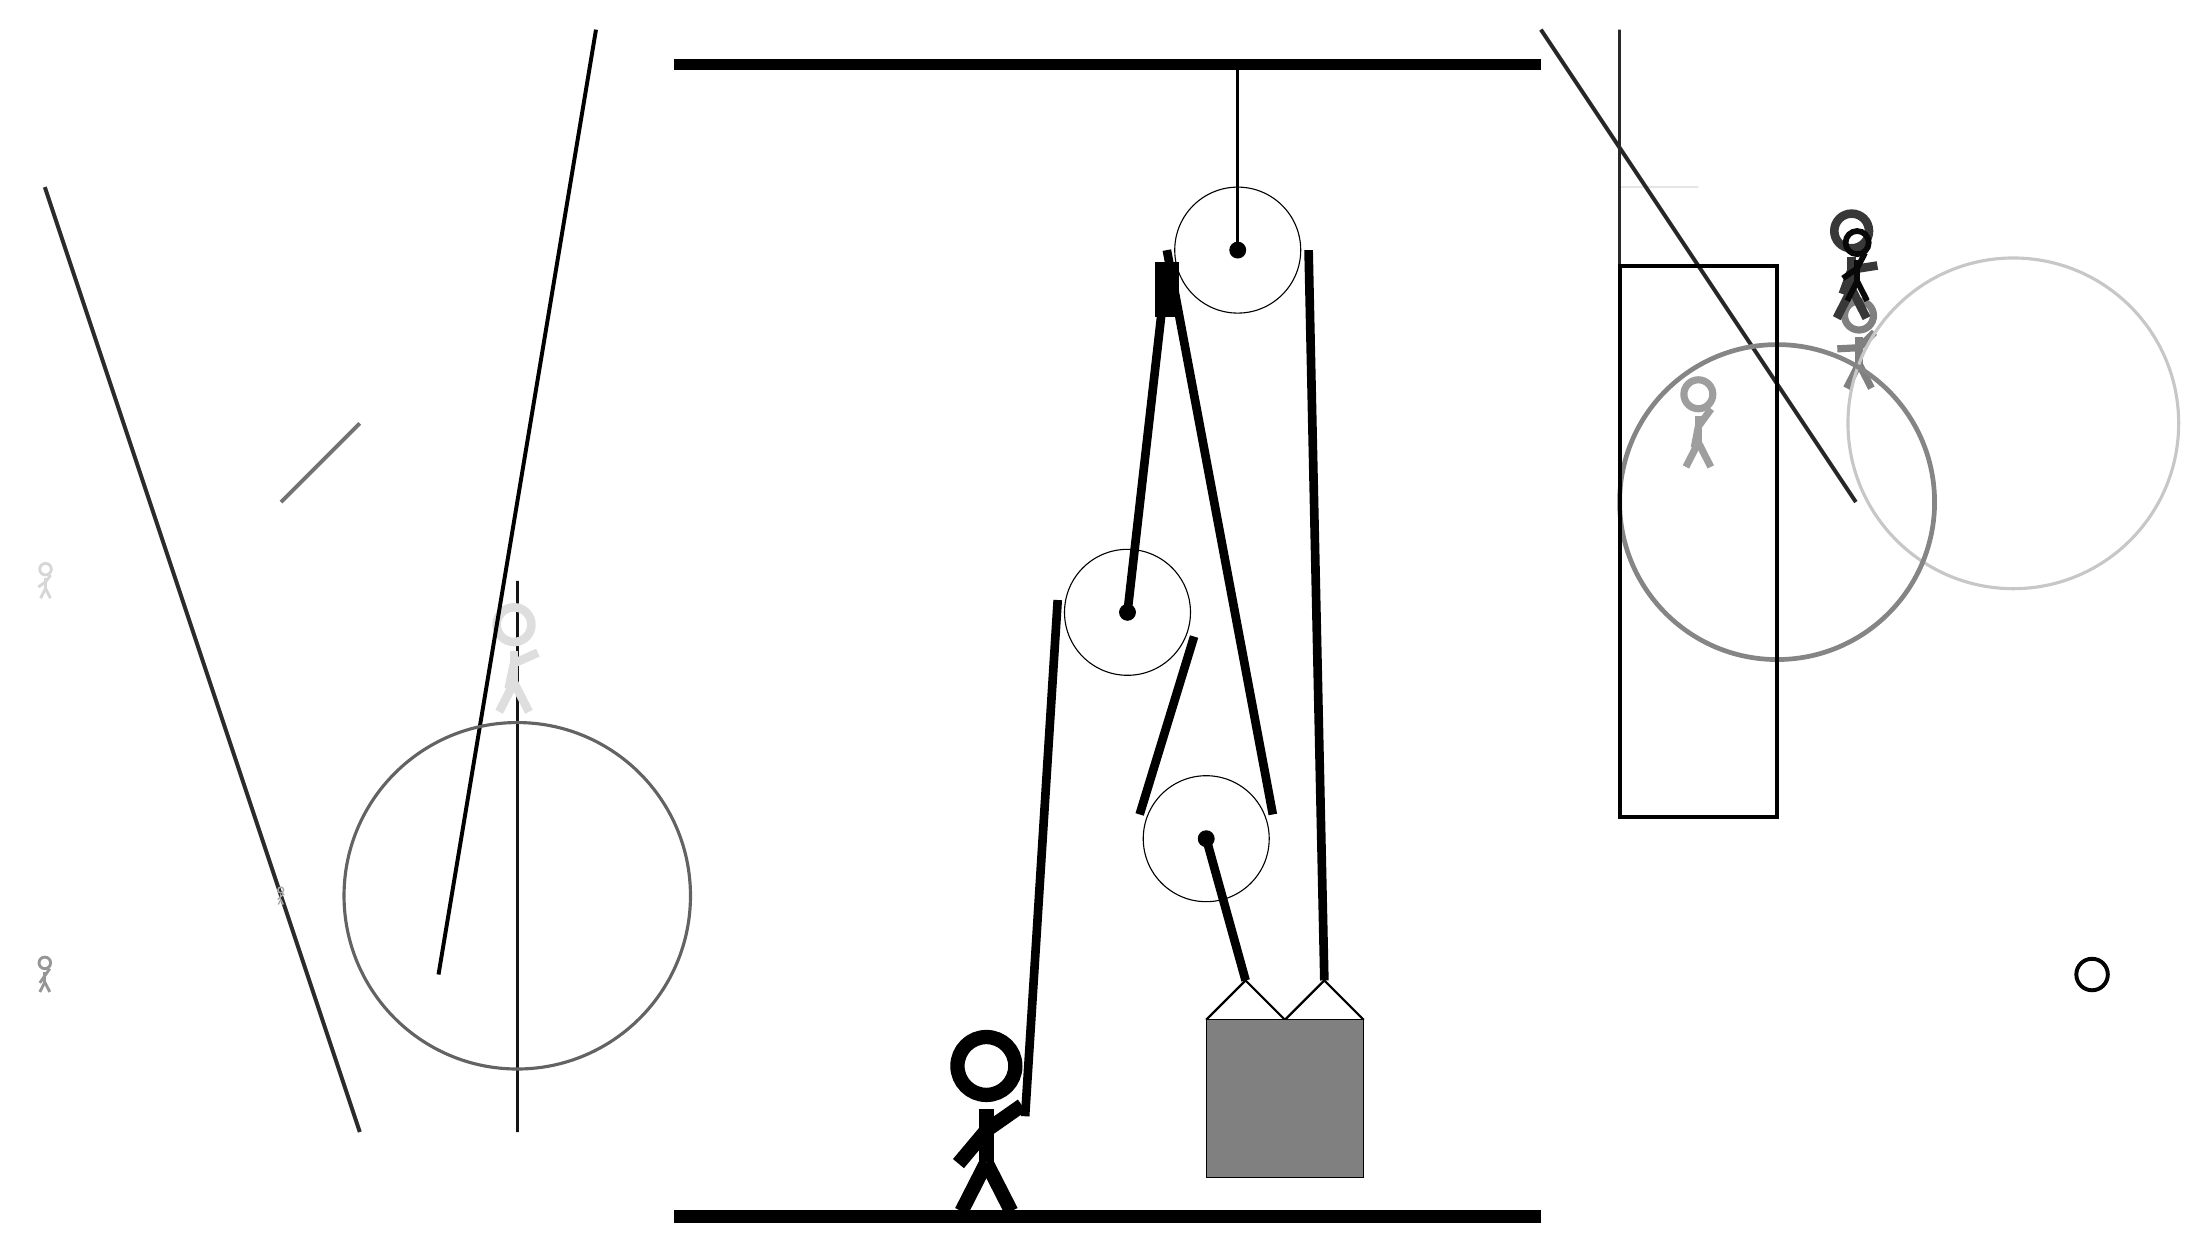
\begin{tikzpicture}
			%%%%% START %%%%%
			
			\draw[fill=black] (-6, 11.5) rectangle (5, 11.625);
			
			\draw (-0.25, 4.6) circle (0.8);
			\draw[fill=black] (-0.25, 4.6) circle (0.1);
			
			\draw[line width=0.5mm, color=black!83](-10, -2) -- (-14, 10);
			
			\node[line width=0.5mm, color=black!16] at (-14, 5) {\Strichmaxerl[2][34][54]};
			\node[line width=0.7mm, color=black!41] at (-14, 0) {\Strichmaxerl[2][55][55]};
			\node[line width=0.6mm, color=black!50] at (9, 8) {\Strichmaxerl[5][3][45]};
			\draw[line width=0.4mm, color=black!92] (-8, 5) rectangle (-8, -2);
			\node[line width=0.4mm, color=black!34] at (-11, 1) {\Strichmaxerl[1][48][38]};
			\draw [line width=0.4mm, color=black!22](11, 7) circle (2.1);
			\draw [line width=0.5mm, color=black!99](12, 0) circle (0.2);
			\node[line width=0.5mm, color=black!38] at (7, 7) {\Strichmaxerl[5][79][54]};
			\draw[line width=0.2mm, color=black!10] (6, 10) rectangle (7, 10);
			\draw[line width=0.5mm, color=black!85](9, 6) -- (5, 12);
			
			\draw [line width=0.6mm, color=black!48](8, 6) circle (2.0);
			\node[line width=0.5mm, color=black!13] at (-8, 4) {\Strichmaxerl[6][78][24]};
			
			\node[line width=0.4mm, color=black!78] at (9, 9) {\Strichmaxerl[6][70][9]};
			\node[line width=0.4mm, color=black!97] at (9, 9) {\Strichmaxerl[4][35][63]};
			\draw[line width=0.3mm, color=black!84] (6, 6) rectangle (6, 12);
			
			\draw[line width=0.5mm, color=black!100] (6, 2) rectangle (8, 9);
			\draw[line width=0.5mm, color=black!100](-7, 12) -- (-9, 0);
			\draw [line width=0.4mm, color=black!61](-8, 1) circle (2.2);
			\draw[line width=0.5mm, color=black!55](-10, 7) -- (-11, 6);
			
			\draw (0.75, 1.725) circle (0.8);
			\draw[fill=black] (0.75, 1.725) circle (0.1);
			
			\draw (1.15, 9.2) circle (0.8);
			\draw[fill=black] (1.15, 9.2) circle (0.1);
			\draw[very thick] (1.15, 9.2) -- (1.15, 11.5);
			
			\draw[thick]  (0.75, -0.575) -- (1.25, -0.075) -- (1.75, -0.575) -- (2.25, -0.075) -- (2.75, -0.575);
			\draw[fill=black!50] (0.75, -0.575) rectangle (2.75, -2.575);
			
			\draw[line width=1.1mm] (-0.25, 4.6) -- (0.25, 9.0);
			\draw[line width=1.1mm, fill=black](0.15, 8.4) rectangle (0.35, 9.0);
			\draw[line width=1.1mm] (-1.55, -1.8) -- (-1.1363, 4.7562);
			\centerarc[line width=1.1mm](-0.25, 4.6)(-20:170:0.9);
			\draw[line width=1.1mm] (0.5957, 4.2922) -- (-0.0957, 2.0328);
			\centerarc[line width=1.1mm](0.75, 1.725)(160:380:0.9);
			\draw[line width=1.1mm] (1.5957, 2.0328) -- (0.25, 9.2);
			\draw[line width=1.1mm](0.75, 1.725) -- (1.25, -0.075);
			\centerarc[line width=1.1mm](1.15, 9.2)(0:180:0.9);
			\draw[line width=1.1mm] (2.05, 9.2) -- (2.25, -0.075);
			
			\node at (-2, -1.9) {\Strichmaxerl[10][50][35]};
			
			\draw[fill=black] (-6, -3) rectangle (5, -3.15);
			
			%%%%% END %%%%%
		\end{tikzpicture}
	\end{figure}	
\end{document}